\documentclass[11pt]{article}
\usepackage[margin=0.8in]{geometry}
\usepackage[T1]{fontenc}
\usepackage{lmodern}
\usepackage{graphicx}
\usepackage{booktabs}
\usepackage{xcolor}
\usepackage{listings}
\usepackage{hyperref}
\usepackage{float}
\definecolor{codebg}{HTML}{F6F8FA}
\definecolor{codekw}{HTML}{2457A6}
\definecolor{codestr}{HTML}{A31515}
\definecolor{codecom}{HTML}{547547}
\lstset{language=Python,basicstyle=\ttfamily\small,backgroundcolor=\color{codebg},
 keywordstyle=\color{codekw}\bfseries,stringstyle=\color{codestr},
 commentstyle=\color{codecom}\itshape,showstringspaces=false,breaklines=true,
 frame=single,rulecolor=\color{black!18},columns=fullflexible}
\title{Intervention Study - Revealing the dominant strategy (truth-telling in SPSB)}
\author{EDSL shared-state experiment setup}
\date{\today}
\begin{document}
\maketitle
\begin{abstract}
This standalone document specifies the shared-state implementation and planned
execution for this archived llm-auction condition. It is a setup paper: no new
inference has been run for this condition, so it reports no model outcomes.
\end{abstract}
\section{Condition and protocol}
Intervention Study - Revealing the dominant strategy (truth-telling in SPSB). This condition uses
3 bidders, private values, and
50 configured auction repetitions with model gpt-4o
at temperature 0.5. Bidders submit sealed bids concurrently against a shared snapshot. The state machine withholds bid records until all required bids arrive, then settles the auction in one close transition.

\begin{table}[H]\centering\begin{tabular}{ll}\toprule
Item & Setup \\\midrule
Condition & intervention\_dominant\_strategy \\
Bidders & 3 \\
Value model & private \\
Configured repetitions & 50 \\
Model & gpt-4o \\
Temperature & 0.5 \\
Inference status & Not run; this file is a setup paper \\
Machine & Defined; diagram generated from EDSL Machine.show\_diagram() \\
\\bottomrule\end{tabular}\caption{Experiment setup; no inference results are included.}\end{table}

\section{Shared-state machine}
Each repetition has its own scope in the shared-state map. The machine definition
is $M=(C,X,A,V,\delta,\kappa)$: constants $C$, internal state $X$, action
interface $A$, public view $V$, action transition $\delta$, and close transition
$\kappa$. Separate scopes ensure that a transition in auction $r$ cannot alter
auction $r'$. The state stores bid records $B=\{(i,s_i,v_i,c_i,b_i)\}$. At close they are sorted by $(-b_i,s_i)$; the configured order selects the settlement bid. In first-, second-, or third-price auctions only the winner pays that bid; in all-pay every bidder pays their own bid. Utility is value less payment.
\begin{figure}[H]\centering
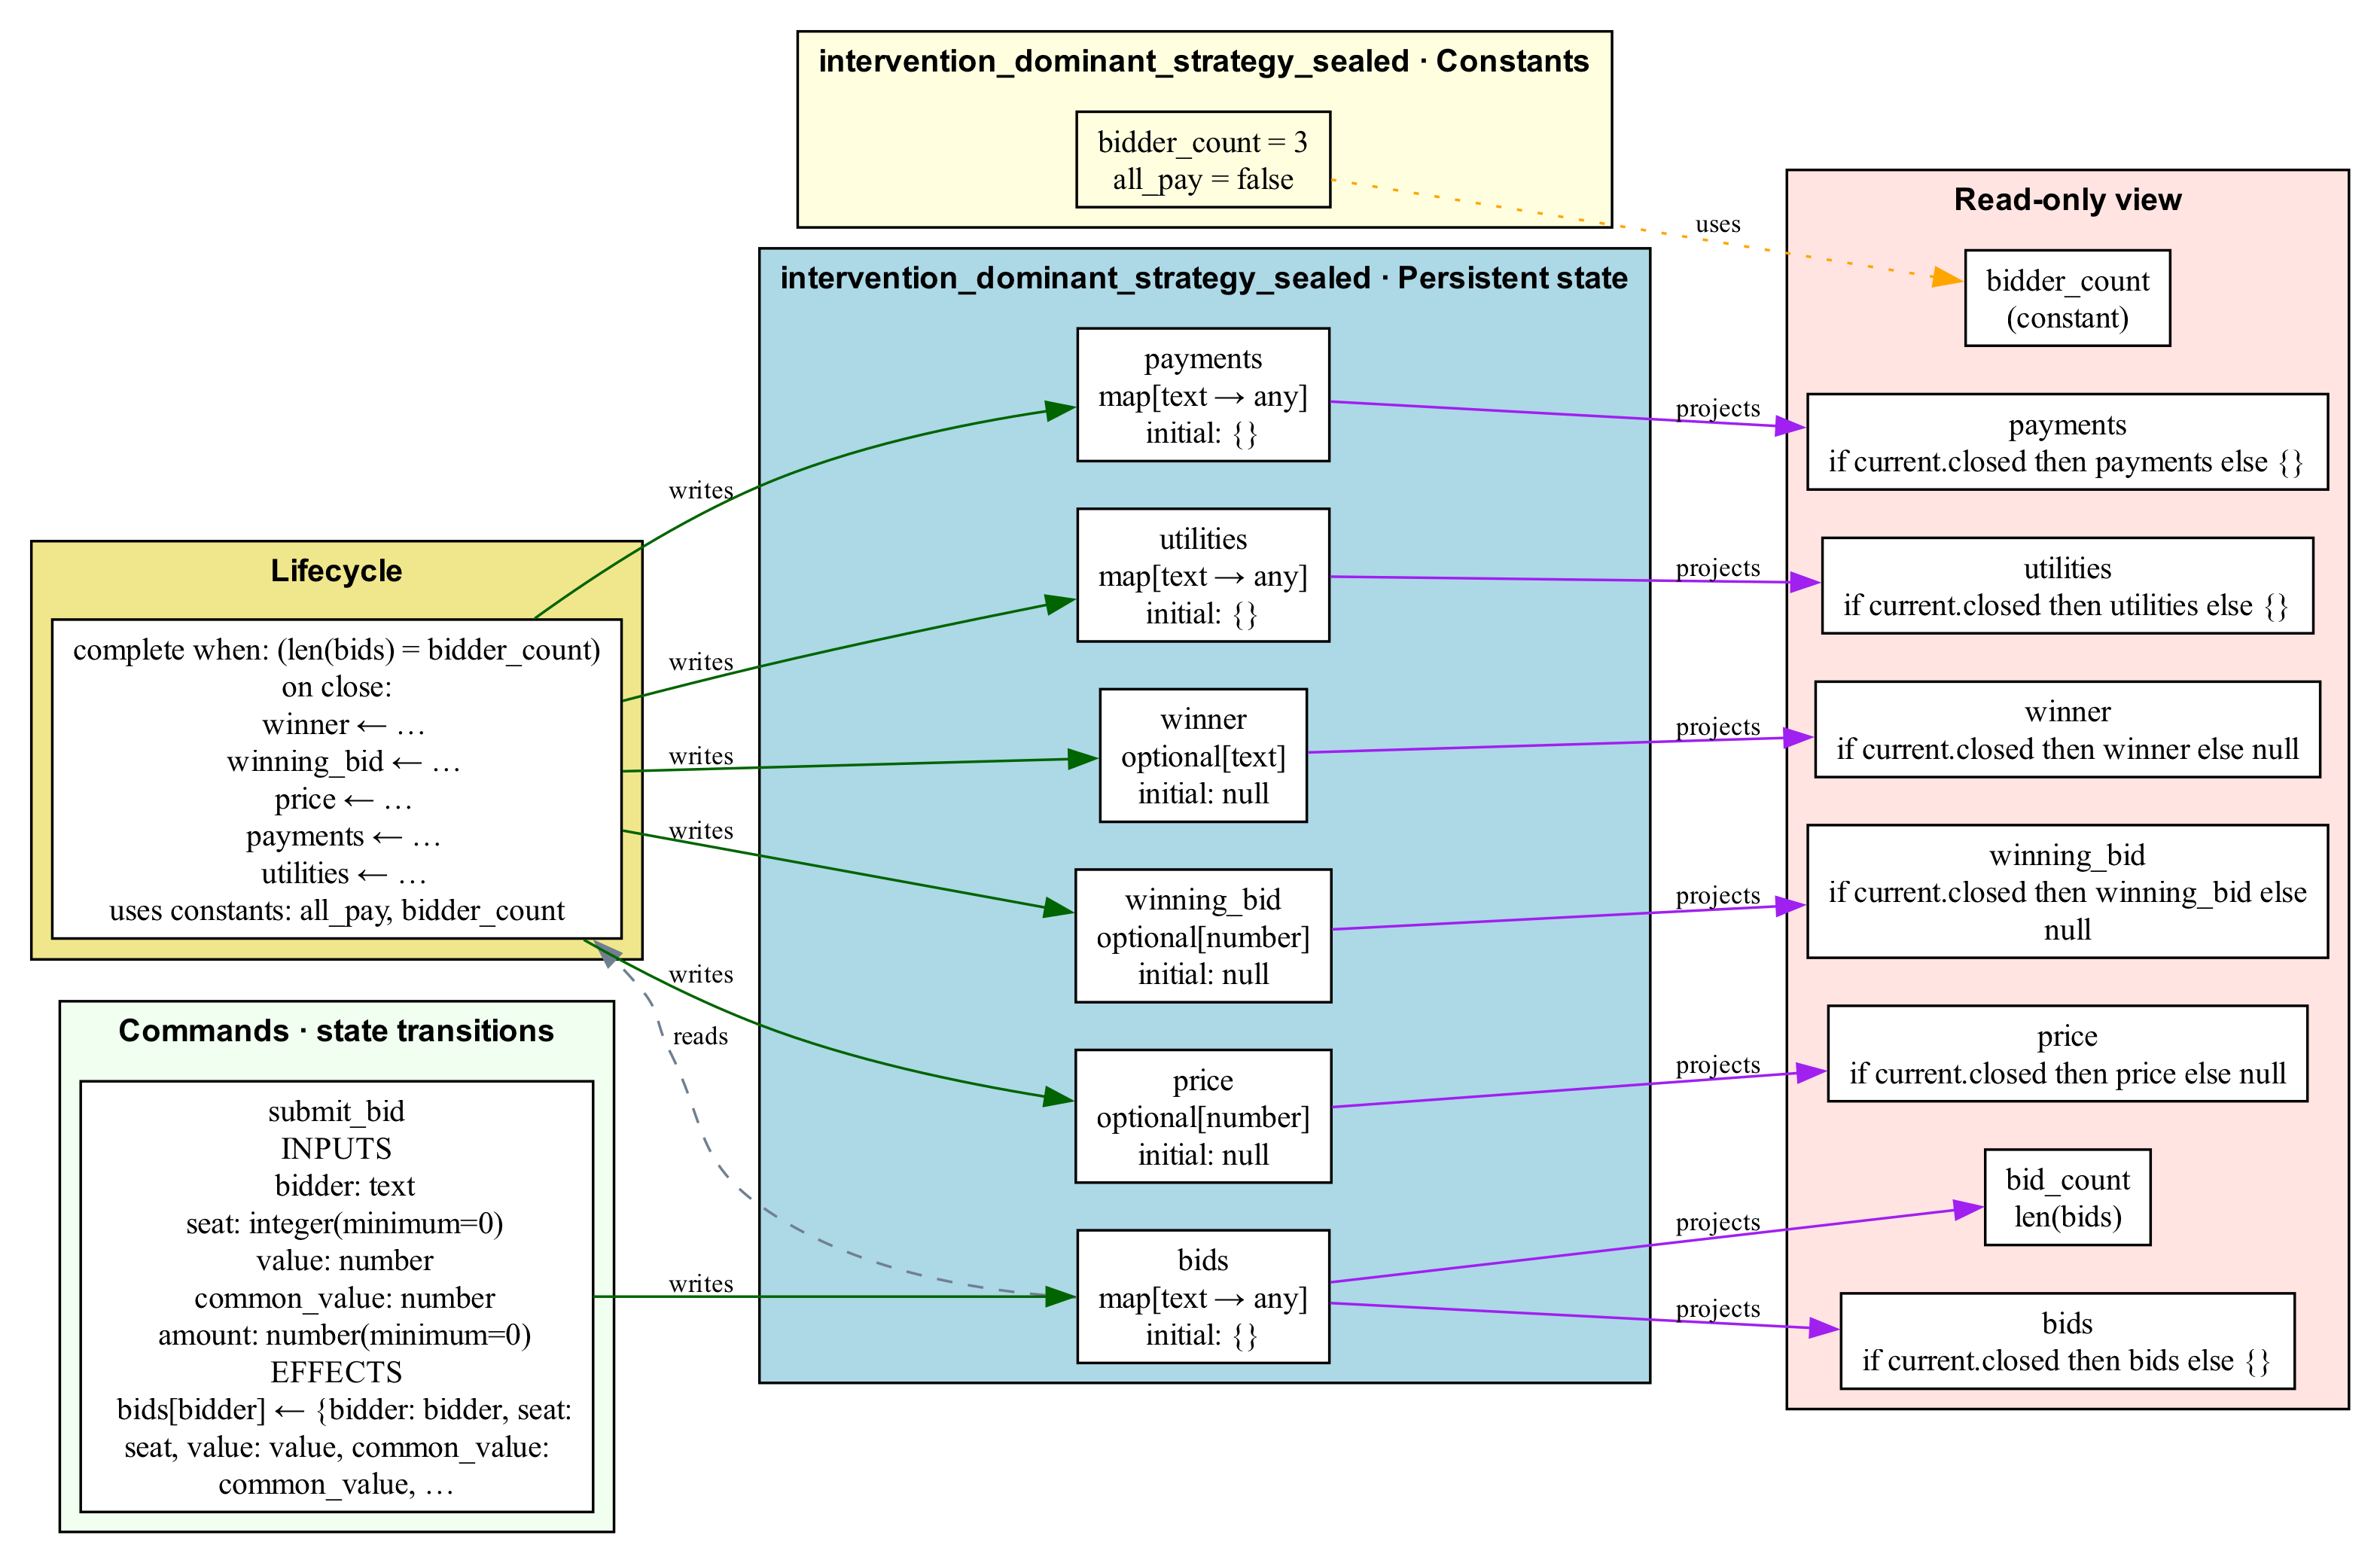
\includegraphics[width=\linewidth]{figures/state_machine.png}
\caption{Diagram generated by EDSL's \texttt{Machine.show\_diagram()}.}
\end{figure}
\subsection{Python machine factory}
The following is the implementation used to build this condition's machine.
\lstinputlisting{machine_definition.py}

\section{Launch command}
The EDSL runner executes locally and uses the model service and key configured
for this experiment. This setup step did not launch interviews. To run the
configured number of repetitions:
\begin{lstlisting}[language=bash]
python -m edsl_replication.shared_state_auctions \\
  configs/experiments/03\_05\_intervention\_dominant\_strategy.yaml \\
  --output edsl_replication/studies/intervention\_dominant\_strategy/raw_results.json
\end{lstlisting}
\section{Results}
Results are pending. After inference, the condition report will be rebuilt from
the EDSL result object, interview answers, machine event history, and exit
snapshots. No outcome estimates or charts are included in this setup paper.
\end{document}
